\DeclareUnicodeCharacter{2028}{} 
\documentclass{article}
\usepackage{blindtext}
\usepackage[T1]{fontenc}
\usepackage[utf8]{inputenc}
\usepackage{titling}
\usepackage{tikz}
\usetikzlibrary{calc}
\usetikzlibrary{arrows.meta}
\usepackage{graphicx}


\title{ Requirements Analysis and Specifications Document\\2020-2021}
\author{Alessandro Polidori (Codice persona 10573078)\\Olimpia Rivera (Codice persona 10617517)}
\date{}



\renewcommand{\contentsname}{Table of Contents}


\begin{document}

\begin{figure}[]
  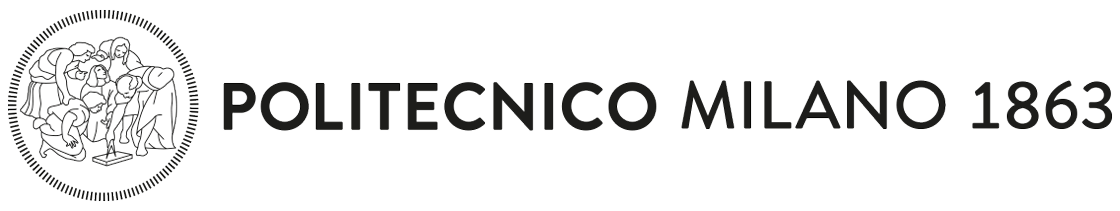
\includegraphics[width=\linewidth]{logo_politecnico.png}
  
\end{figure}
\maketitle
\tableofcontents{}

\newpage

\section{Introduction}

\subsection{Purpose}
This document provides an analysis of the system in terms of assumptions, functional and non functional requirements needed to fulfill its main goals. It describes the domain in which the system will be deployed by presenting relevant scenarios and use cases and it highlights the software’s limits and constraints.
\bigskip\\
The document is addressed to all the stakeholders affected by the software and is meant to be used by developers in order to realize a system that meets the purpose for which it was intended.\\

\subsection{Scope}
\subsubsection{Description of the given problem}
The CLup system is designed to regulate accesses to stores and manage lines in real time in order to respect restrictions imposed by the virus emergency and avoid crowds and long lines. In particular, the software is offered to both stores managers to monitor the influx of people in their buildings and to common users, allowing them to virtually “line-up” from home and book visits to the stores.\\
\smallskip\\
The main functionalities offered by CLup are the following:\\
\begin{itemize}
\item Basic service: allows stores' customers to line up from home and to approach the store only when their turn is about to arrive. In order for this lining up mechanism to work effectively, the software generates an estimation of the waiting time and alerts users when is the moment to reach the store, taking into account the time they need to get to the shop from the place they are located. The estimated time is calculated considering the number of people in the virtual line and the time spent inside the store by the costumers that are already shopping. The system is also able to recalculate the waiting times of users in the queue and manage the line in the event that someone does not show up when her/his turn is arrived or decides to cancel her/his reservation. In addiction, when customers enter and exit the stores, a QR code generated by the application is scanned, allowing store managers to monitor entrances.
\item Advanced service: allows users to book a time-slot to visit the store. When booking users can indicate the list (or at least the categories) of the items that they intend to purchase. The system will be able to manage visits in a finer way taking into account the store's departments that customers are going to occupy.
\end{itemize}
When customers line up or make a reservation they have to provide the expected duration of the visit or let the software itself infer it (this works only for long-term customers by analyzing the customer’s previous visits).
Be aware that the functions described above will be further detailed in the next sections of the document.
\subsubsection{World Phenomena}
\noindent\medskip
[WP1] - Stores’ customers either owning or not a smartphone.\\
\noindent\medskip
[WP2] - Customers approaching the store.\\
\noindent\medskip
[WP3] - Customers arriving too early at the shop for unexpected reasons.\\
\noindent\medskip
[WP4] - Customers doing the shopping.\\
\noindent\medskip
[WP5] - Customers walking away from store.
\subsubsection{Shared Phenomena}
\noindent\medskip
[SP1] - User enters the store (QR code scanned) - World controlled.\\
\noindent\medskip
[SP2] - User gets in line - World controlled.\\
\noindent\medskip
[SP3] - System shows number and estimated waiting time - Machine controlled.\\
\noindent\medskip
[SP4] - System generated QR code and line number - Machine controlled.\\
\noindent\medskip
[SP5] - System notifies the user to reach the store - Machine controlled.\\
\noindent\medskip
[SP6] - System updates waiting time - Machine controlled.\\
\noindent\medskip
[SP7] - User doesn't arrive in time - World controlled.\\
\noindent\medskip
[SP8] - User cancels reservation (either slot or line) - World controlled.\\
\noindent\medskip
[SP9] - User books a slot - World controlled.\\
\noindent\medskip
[SP10] - User indicates expected duration of visit or requests system to infer it - World controlled.\\
\noindent\medskip
[SP11] - User makes list of items - World controlled.\\
\noindent\medskip
[SP12] - User exits the store (QR code scanned) - World controlled.\\
\subsubsection{Goals}
\noindent\medskip
[G1] - Provide customers a safe environment in the stores.\\
\noindent\medskip
[G2] - Manage virtual lines in order to avoid the formation of long lines outside stores.\\
\noindent\medskip
[G3] - Allow store managers to monitor the influx of people in their buildings.\\
\noindent\medskip
[G4] - Allow users to book slots for visiting the store.\\
\noindent\medskip
[G5] - Allow users to arrive on time for their turns.\\
\subsection{Definitions, Acronyms, Abbreviations}
\subsubsection{Definitions}
\subsubsection{Acronyms}
\subsubsection{Abbreviations}

\subsection{Reference Documents}
\subsection{Overview}
The RASD document is structured in the following 5 chapters:
\begin{itemize}
\item\textbf{Chapter 1} describes the document’s purpose and brief identification of the context in which the application is going to work given its main functionalities. It also provides lists of world phenomena, shared phenomena and goals that the system is supposed to achieve. Finally, useful specifications (definitions, acronyms, abbreviations) are included for a better understanding of the next sections of the document.
\item\textbf{Chapter 2} gives an overall description of the project. The class diagram in the Product Perspective provides a conceptual overview of the main elements of the system and the state charts describe the evolution of relevant objects. In the Product Function section, the system’s high level functionalities are further detailed and clarified. The expected type of actors that will interact with the system are listed in User Characteristics. Ultimately, chapter 2 describes the system’s constraints and the domain properties assumed to hold in the world.
\item\textbf{Chapter 3}
\item\textbf{Chapter 4}
\item\textbf{Chapter 5}
\end{itemize}


\section{Overall Description}
\subsection{Product Perspective}
The class diagram below gives a high level representation of the system domain. Classes contains only attributes necessary to clarify the most important dynamics. \textbf{QR Code} is associated either to a \textbf{Turn Number} or to a \textbf{Reservation} and has attributes required to associate the measured duration of the stay to the user.
\begin{figure}[]
  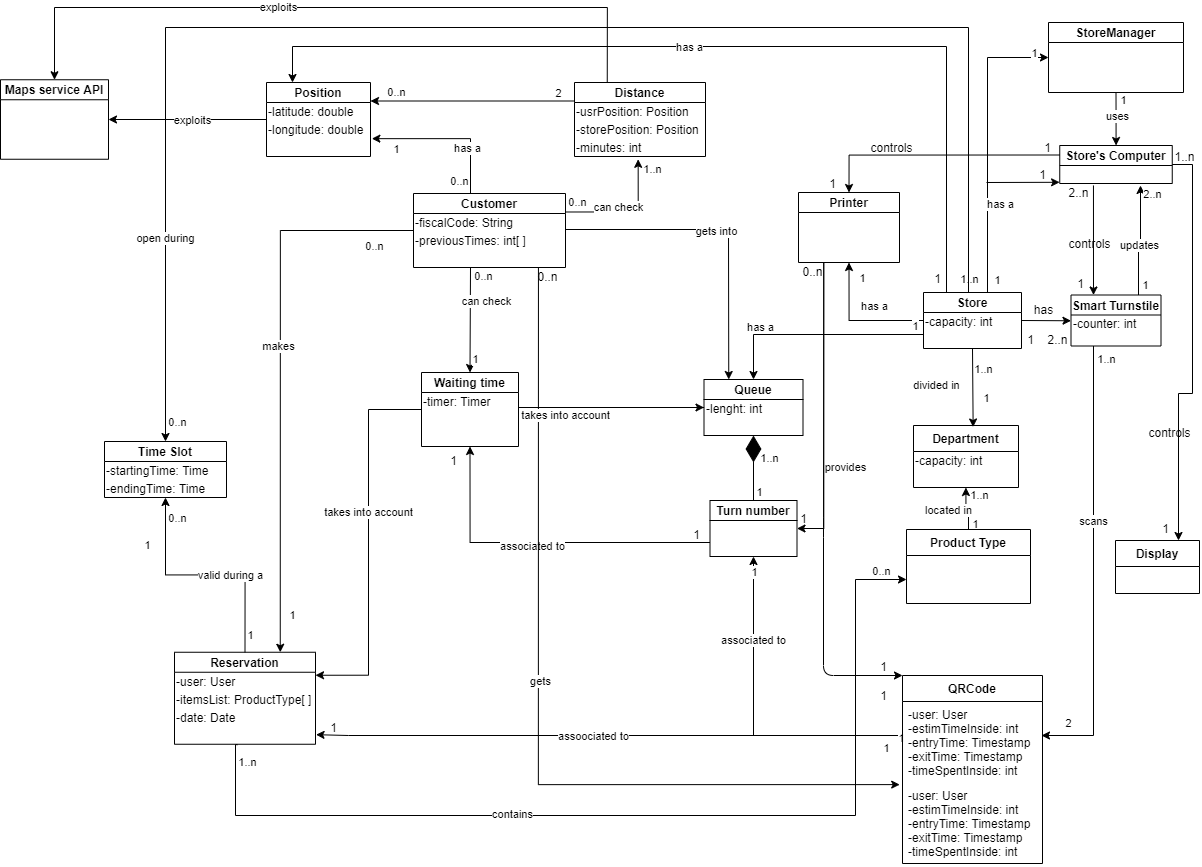
\includegraphics[width=\linewidth]{class_diagram.png}
  
\end{figure}

\subsection{Product Functions}
The main functions that the system will provide are listed in the following section. The identified high level requirements will be further broken down and detailed in section 3, with respect to the previously recognized goals of the system.
\subsubsection{Line up} 
\subsubsection{Book a visit} 
\subsubsection{Keep track of accesses} 
\subsubsection{Line up} 
\subsection{User Characteristics}
\subsection{Constraints}
The system will have to ask users' permission to retrieve and use their positions without storing them. Moreover, the system will manage and safely store information about users' visits durations.
\subsection{Assumptions and Dependancies}
\subsubsection{Domain assumptions}
\noindent\medskip
[D1] - GPS provides the exact location with an error of 5 meters at most.\\
\noindent\medskip
[D2] - The time calculated from Google Maps to reach the store is correct.\\
\noindent\medskip
[D3] - The user does not to arrive earlier than the indicated time.\\
\noindent\medskip
[D4] - The user follows the shortest path to the store, without making deviations and stops.\\
\noindent\medskip
[D5] - Each reservation is meant to be for one and only one person.\\
\noindent\medskip
[D6] - The turnstiles let you in or out only if the scanned QR code is valid.\\
\noindent\medskip
[D7] - The user doesn't change location while is waiting for his/her turn.\\



\end{document}